\begin{figure}[ht]
%{0.45\textwidth}
  \centering
%  \resizebox{\linewidth}{!}{
\begin{adjustbox}{max size={.49\textwidth}}
    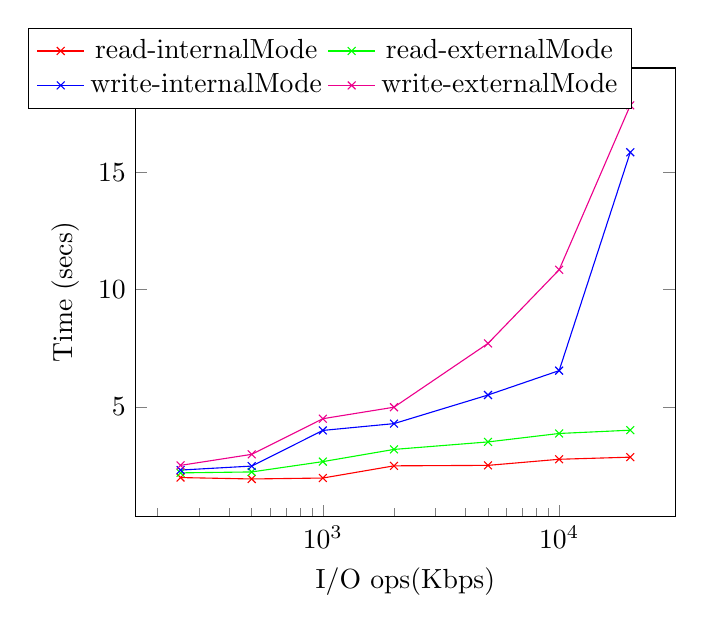
\begin{tikzpicture}
      \begin{axis}[
        xmode=log,
        legend style={at={(-0.2,1.09)},anchor=north west,legend columns=2},
        xlabel=I/O ops(Kbps),
        ylabel=Time (secs)]
        \addplot[color=red,mark=x] coordinates {
          (0,1.85)
          (250,1.99)
          (500,1.93)
          (1000,1.97)
          (2000,2.49)
          (5000,2.51)
          (10000,2.77)
          (20000,2.86)
        };
        \addlegendentry{read-internalMode}
        \addplot[color=green,mark=x] coordinates {
          (0,1.97)
          (250,2.19)
          (500,2.23)
          (1000,2.67)
          (2000,3.19)
          (5000,3.51)
          (10000,3.87)
          (20000,4.01)
        };
        \addlegendentry{read-externalMode}				
        \addplot[color=blue,mark=x] coordinates {
          (0,1.85)
          (250,2.31)
          (500,2.48)
          (1000,4.00)
          (2000,4.29)
          (5000,5.51)
          (10000,6.55)
          (20000,15.86)
        };
        \addlegendentry{write-internalMode}				
        \addplot[color=magenta,mark=x] coordinates {
          (0,1.87)
          (250,2.51)
          (500,2.98)
          (1000,4.50)
          (2000,4.99)
          (5000,7.71)
          (10000,10.85)
          (20000,17.86)
        };
        \addlegendentry{write-externalMode}
      \end{axis}
    \end{tikzpicture}
  \end{adjustbox}
%  }
  \captionsetup{justification=centering}
  \caption{Live Cloning suspend time with increasing amounts of I/O operations }
  \label{fig:fioResults}
\end{figure}


\noindent
\textbf{Micro Benchmark using I/O operations:}
%To understand the impact of cloning in further detail, we ran a micro-benchmark of an I/O application to see how well cloning scales.
%As explained earlier, the cloning process can be divided into two parts: an rsync operation which does an ``pre-copy'' of the VM, and a follow-up rsync operation while the target container is suspended, to make sure that both the production and test containers have the exact same state.
%The idea is to reduce the time taken to suspend the production container, so that it has minimal impact on the user.
The main factor that impacts suspend time is the number of ``dirty pages'' in the suspend phase, which have not been copied over in the pre-copy rsync operation (see section~\ref{sec:CloneManager}).
To understand this better, we use fio (flexible I/O tool for Linux)~\cite{fio}, to gradually increase the number of I/O operations while doing live cloning.
Fio reads or writes random values in a file with a rate controlled I/O bandwidth as specified by the user. 
The suspend time is observed by instrumentation within the cloning script, which reports time taken by each of the suspend processes.
Additionally, we ensure that the I/O job being processed by fio is long enough to last through the entire cloning process.

We found that in comparison to write, read operations have a much smaller impact on suspend time of live cloning.
This can be attributed to the increase of ``dirty pages'' in write operations, whereas for read, the disk image remains largely the same.
We also found, that internal mode is much faster than external mode, as both the production and debug-container are hosted in the same physical device.
We believe, that for higher I/O operations, with a large amount of ``dirty-pages'', network bandwidth becomes a bottleneck: leading to longer suspend times.
Overall, the internal mode is able to manage write operation up-to 10 mbps, with a total suspend-time of approx 5 seconds.
Whereas, the external mode is only able to manage upto 5-6 mbps, for a 5 sec suspend time.

%This in turn depends on I/O operations happening in the container.
%Naturally, write operations, and in memory pages in the container while cloning the container, will increase the number of dirty pages, and increase the time of the suspend operation.
%Here we also compare the performance of cloning in the internal mode vs the external mode, while showing the time taken in various stages of cloning.
%While for lower I/O operations, the performance of both were similar, as we go higher, the external mode which uses the network to transfer the dirty pages during the cloning operations becomes a bottleneck. 
%We also observed that the majority of the time is spent in pcopy after suspend, which is doing the copy of the dirty bits after suspend, especially for higher I/O's the other operations become negligible in comparison.
%For relatively lower I/O operations, "live cloning" takes only a few seconds (~2/3 secs) and is not disruptive to application clients (there is no loss of service visible). 
%However, in high I/O intensive workloads, the amount of time taken to clone can go up exponentially, and will lead to dropping of requests.
%In such cases, we did observe a few retries and in HTTP but no timeouts, naturally the performance of the server did suffer. 
